%--------------------
% Packages
% -------------------
\documentclass[11pt,a4paper]{article}
\usepackage[utf8x]{inputenc}
\usepackage[T1]{fontenc}
%\usepackage{gentium}
\usepackage{mathptmx} % Use Times Font


\usepackage[pdftex]{graphicx} % Required for including pictures
\usepackage[swedish]{babel} % Swedish translations
\usepackage[pdftex,linkcolor=black,pdfborder={0 0 0}]{hyperref} % Format links for pdf
\usepackage{calc} % To reset the counter in the document after title page
\usepackage{enumitem} % Includes lists

\frenchspacing % No double spacing between sentences
\linespread{1.2} % Set linespace
\usepackage[a4paper, lmargin=0.1666\paperwidth, rmargin=0.1666\paperwidth, tmargin=0.1111\paperheight, bmargin=0.1111\paperheight]{geometry} %margins
%\usepackage{parskip}

\usepackage[all]{nowidow} % Tries to remove widows
\usepackage[protrusion=true,expansion=true]{microtype} % Improves typography, load after fontpackage is selected

\usepackage{lipsum} % Used for inserting dummy 'Lorem ipsum' text into the template

\usepackage{plantuml}

\usepackage{etoolbox} % Adds '\clearpage' to every '\section command' (newpage).
\pretocmd{\section}{\clearpage}{}{} 


%-----------------------
% Set pdf information and add title, fill in the fields
%-----------------------
\hypersetup{ 	
pdfsubject = {Program Systems Engineering},
pdftitle = {itssoover},
pdfauthor = {Ignas Časas, Mykolas Marius Budrys, Augustas Kniška}
}

%-----------------------
% Begin document
%-----------------------
\begin{document} %All text i dokumentet hamnar mellan dessa taggar, allt ovanför är formatering av dokumentet

\begin{titlepage}
    \centering
    % Remove page numbering from title
    \thispagestyle{empty}
    
    % University name
    {\Large VILNIAUS UNIVERSITETAS\\
    Matematikos ir informatikos fakultetas}\par
    
    \vspace{3cm} % vertical space
    
    % Title of the work
    {\Large 2\textsuperscript{nd} Laboratory Work}\par
    \vspace{0.5cm}
    {\Large \textbf{itssoover}}\par
    {\Large \textbf{Iteration, design and implementation}}\par
    
    \vspace{3cm}
    
    % Authors
    {\large
    Ignas Časas\\
    Mykolas Marius Budrys\\
    Augustas Kniška
    }\par
    
    \vspace{8cm}
    
    % Bottom of the page
    {\large
    Matematikos ir informatikos fakultetas\\
    Vilniaus universitetas\\
    Lietuva
    }\par
    
    \vfill

    \large 2025
    
\end{titlepage}

\section{Context}
 Some text and ideas are mentioned...

\section{Logical View}

\subsection*{Class Diagram}
    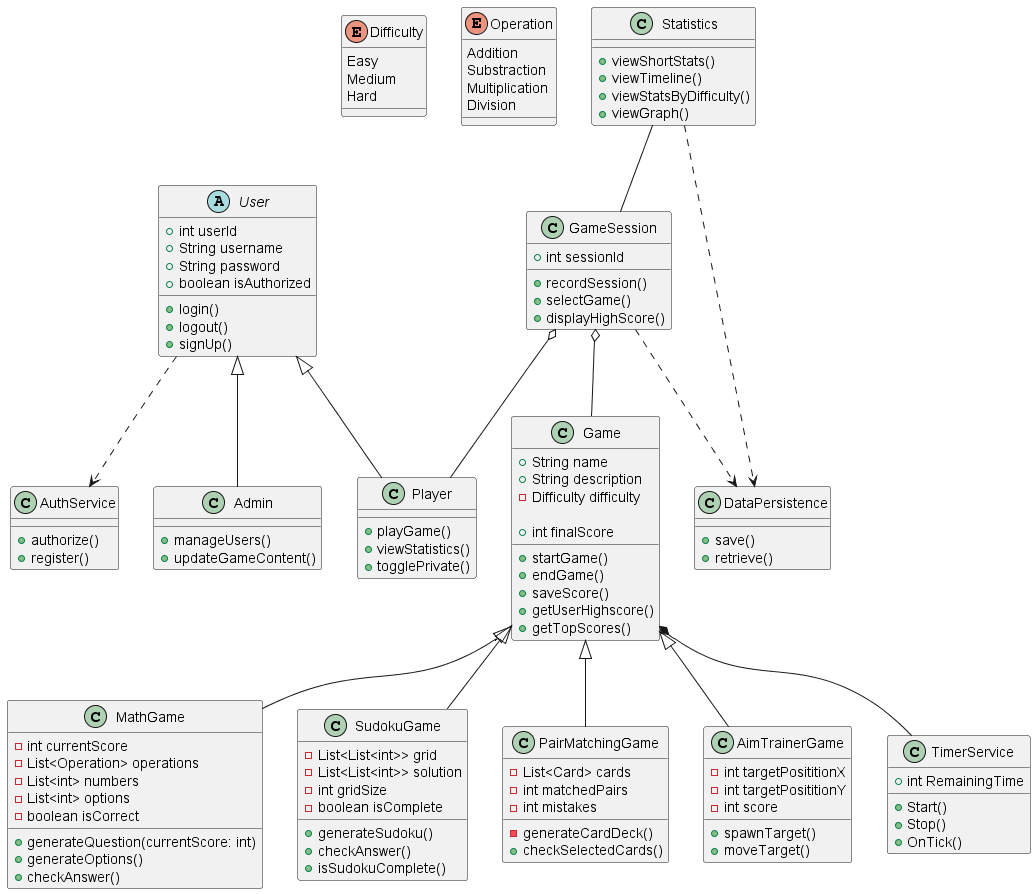
\includegraphics[width=\textwidth]{out/Diagrams/class_diagram/class_diagram.png}

\subsection*{State Diagram}
...State diagram

\section{Development View}

\subsection*{Package Diagram}
...Package diagram

\subsection*{Component Diagram}
...Component diagram

\section{Process View}

\subsection*{Sequence Diagram}
...Sequence diagram

\section{Physical View}

\subsection*{Deployment Diagram}
...Deployment diagram

\section{Use Case View}
...Use cases

\section{Traceability}

%\lipsum[1-3]



\end{document}
